\section{Introduction}

Having studied the details of how matter bends light, now we'll examine how 
to use refraction to form images of various objects.  Lenses are designed to 
refract light rays from an object and focus them into an image. We'll learn 
what the {\it focal length} of a lens is and study the relationship between 
the distance of an object from a lens and the distance of its image, known as 
the {\it thin lens equation}. We'll also see how to use combinations of lenses 
to form images, which is the principle behind microscopes and telescopes.

\section{Theory}

\subsection{References}

Geometric 
optics, the optics of lenses, is covered in Chapter~36 (Geometric Optics). 
Imaging optics and lenses are discussed in Sections~36.3 (Images 
Formed by Refraction) and~36.4 (Thin Lenses).  

\subsection{Imaging Optics and Lenses}

We've learned that the refraction of light at a surface may be described by 
Snell's law.  This behavior is exploited in the design of lenses, which make
use of refraction to focus light rays to form images.  How a lens works is 
fairly simple to explain, but we'll forego any detailed mathematical 
description; we'll also consider only convex, or converging, lenses.  For a 
more comprehensive survey, consult the references to Serway already given.

A converging lens is designed so that parallel rays are focused into a point, 
called the {\it focal point} of the lens, illustrated in 
Figure~\ref{fig:opt:focalpt}.
\begin{figure}[htb]
\centering 
\epsfxsize=8cm 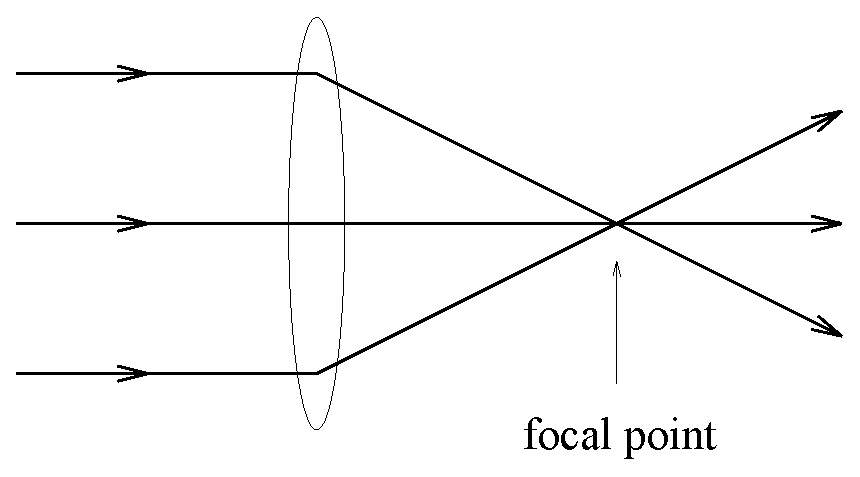
\includegraphics[scale=0.6]{9_imaging/focalpt.eps}
\caption{A converging lens focuses parallel rays.}
\label{fig:opt:focalpt}
\end{figure}
How this happens can be seen by examining part of the lens; in fact we'll look
at only the front surface, in Figure~\ref{fig:opt:frontsurf}.
\begin{figure}[htb]
\centering 
\epsfxsize=8cm 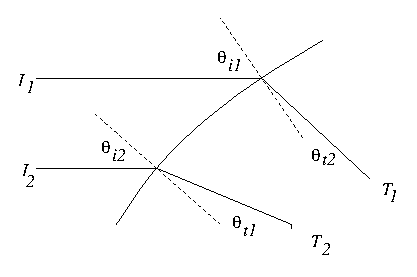
\includegraphics[scale=0.6]{9_imaging/frontsurf.eps}
\caption{The front surface of a lens.}
\label{fig:opt:frontsurf}
\end{figure}
If $I_1$ is incident on the surface with incident angle $\theta_{i1}$, and  $I_2$ is incident on the surface with incidence angle $\theta_{i2}$, keeping in mind that the two incident rays are parallel we can use Snell's law, with the general condition that $n_{\mbox{lens}}>n_{\mbox{air}}$, to show that
the resulting refracted rays $T_1$ and $T_2$ converge.  It is left as another exercise to the 
student to develop this argument further and to draw a sketch of the second
surface of the lens, where $T_1$ and $T_2$ exit the lens into the air, to 
show that the final rays are also converging, as we've indicated in 
Figure~\ref{fig:opt:focalpt}. A lens is made by carefully grinding a piece of
glass (typically) to a precise curvature, so that all of the parallel rays
converge at the same point, namely the focal point of the lens.

The whole reason for using lenses is to convert an object to an image. Why 
this is important is obvious if you consider what a camera does. It takes an 
object that you've taken an interest in and places its image on film, which 
you can preserve for posterity.  Also, as we'll see, the object and image will 
not in general be of the same size. This is important if our object is too 
small or too large to for us to see conveniently with the naked eye.  The 
proper lens will produce an image that allows us to view the object easily. 

Let's examine how we can determine the location of the image produced by a 
lens of an object placed at a known distance.  We'll first learn how to do 
this graphically, then we'll see how to use an equation to help us.  We'll 
illustrate the object and image with arrows, as in 
Figure~\ref{fig:opt:objandim}.
\begin{figure}
\centering 
\epsfxsize=11cm 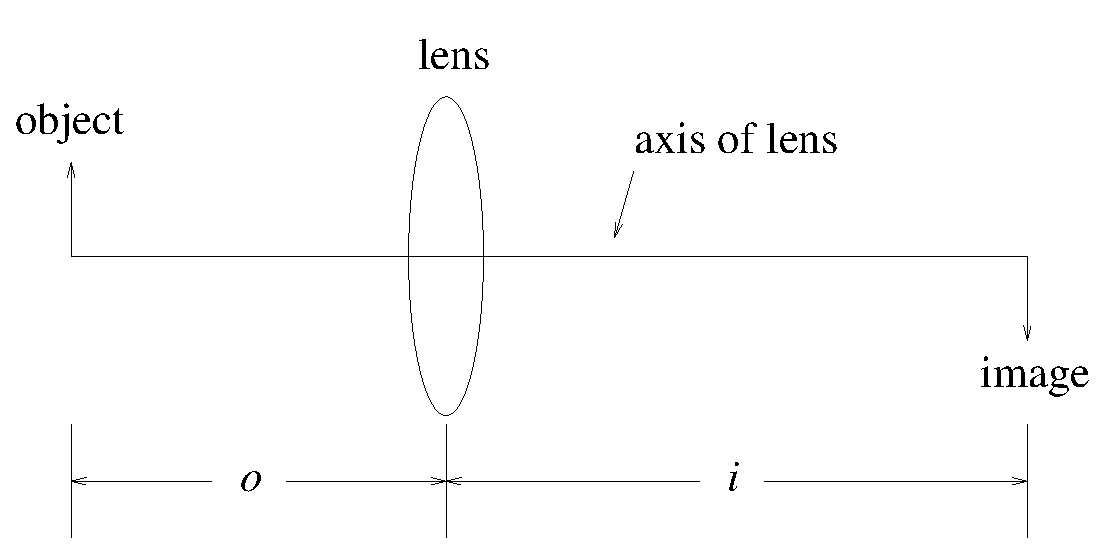
\includegraphics[scale=0.6]{9_imaging/objandim.eps}
\caption{The definition of object and image distances.}
\label{fig:opt:objandim}
\end{figure}
The object distance, $o$, and the image distance, $i$, are defined in the 
figure.  We'll find the image by creating what is called a {\it ray diagram}.
First, we assume that the object is {\it outside} of the focal length of the
lens, or $o>f$, if we use $f$ to denote the focal length. We then draw three
rays, see Figure~\ref{fig:opt:outsidef}.   
\begin{figure}
\centering 
\epsfxsize=13cm 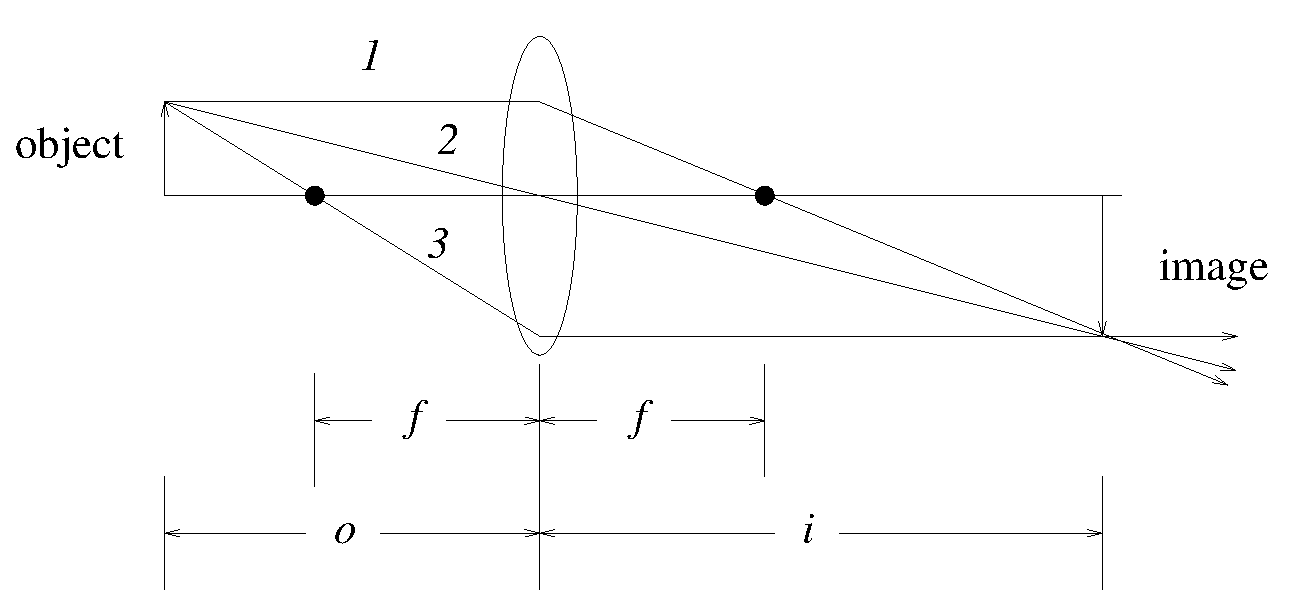
\includegraphics[scale=0.6]{9_imaging/outsidef.eps}
\caption{The ray diagram when the object is outside of a focal length.}
\label{fig:opt:outsidef}
\end{figure}
\begin{figure}
\centering 
\epsfxsize=13cm 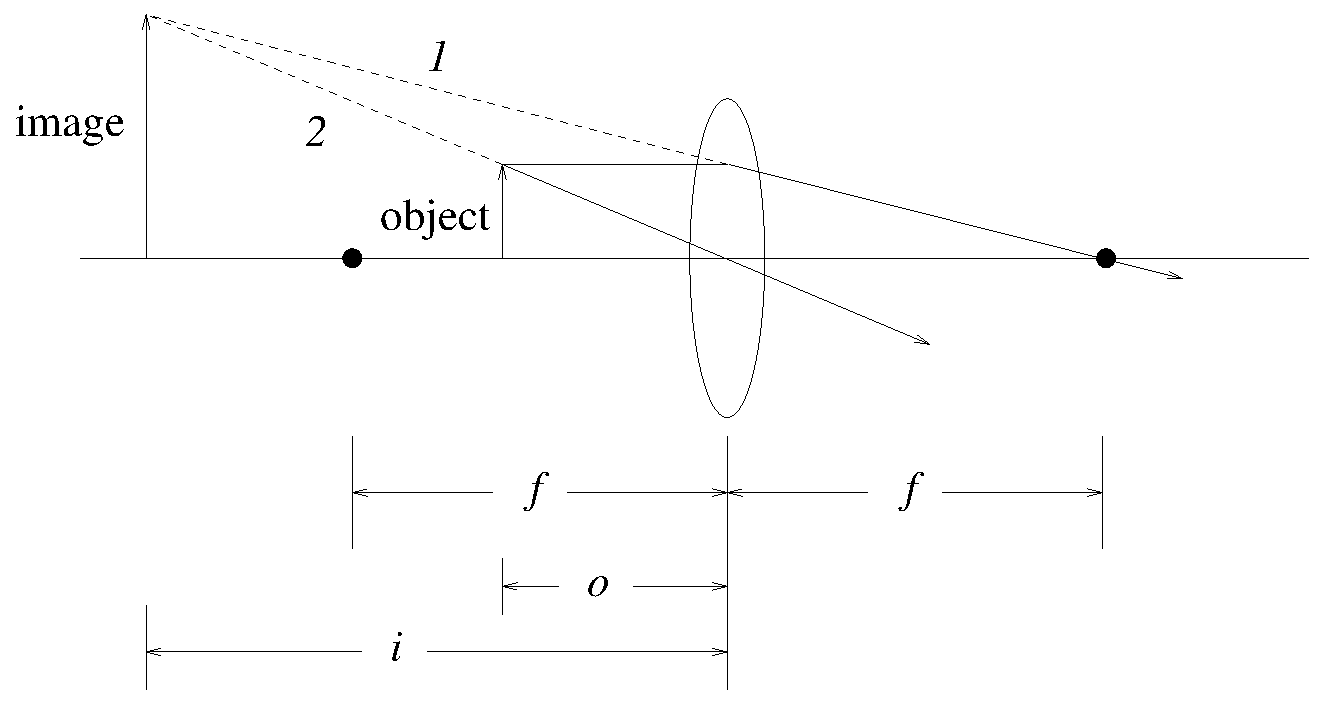
\includegraphics[scale=0.6]{9_imaging/insidef.eps}
\caption{The ray diagram when the object is inside of a focal length.}
\label{fig:opt:insidef}
\end{figure}

Ray~1 is the ray parallel to the axis of the lens, which will be focused 
through the opposite focal point; ray~2 is the ray which passes right through 
the center of the lens; while ray~3 is the opposite of ray~1, it passes through
the near focal point, so that it is focused into a parallel ray.  The image
appears at the {\it intersection} of the three rays.  Of course, you would be 
able to see the image anywhere on the right-hand side of the lens, but it would
be out of focus and blurry unless you were at the image distance.  This image 
is also called a {\it real} image, because you would be able to focus it onto 
a screen held in front of the lens.  Note also that the image is 
{\it inverted}, that is, it's upside-down. If this is a bit confusing now, 
don't worry; we're going to examine each of these statements in the lab.

If the object is {\it inside} of the focal length, $o<f$, things get a bit 
trickier.  The ray diagram is drawn in Figure~\ref{fig:opt:insidef}.
We still draw the parallel ray~1, but we extend the ray {\it backwards}. 
Ray~2 is still the center ray, but again, we extend it backwards.  Where rays~1
and~2 intersect marks the image. Note that the image is on the {\it same side}
of the lens as the object. This image differs from a real image, because
you can't project it on a screen, so we call it {\it virtual}.  You can still
see it by looking through the lens though. Also note that the image is now
rightside-up, we say that it is ``upright.'' 


\subsection{Compound Lenses}

A compound lens is simply a set of several lenses arranged so that the light
from each lens passes through the next, as in Figure~\ref{fig:opt:compounddef}.
\begin{figure}[h]
\centering 
\epsfxsize=14cm 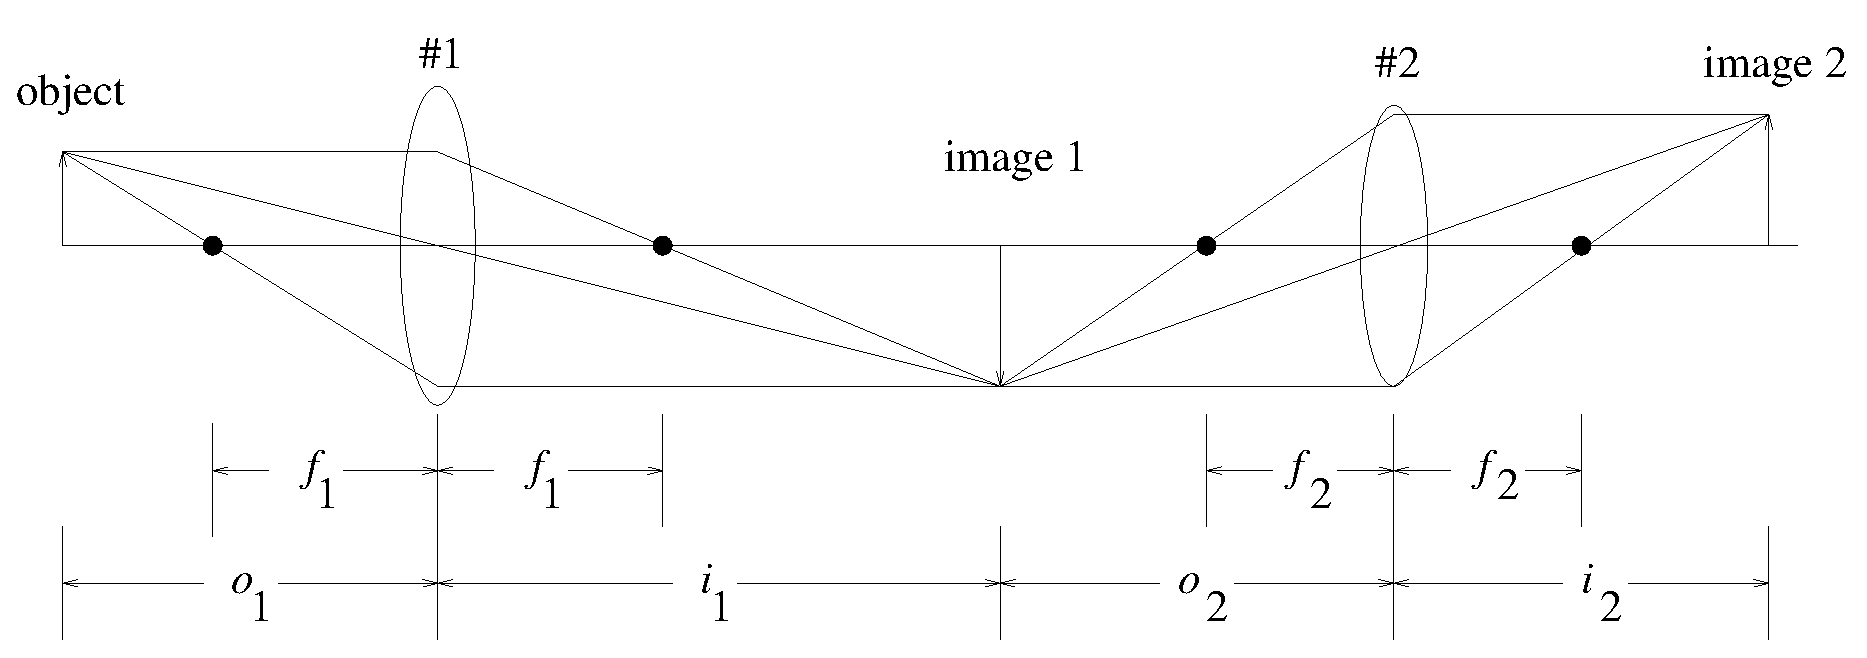
\includegraphics[scale=0.4]{9_imaging/compounddef.eps}
\caption{In a compound lens, the image of the preceding lens acts as the object
for the following lens.}
\label{fig:opt:compounddef}
\end{figure}
The only ``new'' piece of information we need to deal with compound lenses is
that the image produced by one of the lenses will act as the object for the 
next lens in the series. In Figure~\ref{fig:opt:compounddef}, the ray diagram 
for a two-lens system illustrates this principle nicely.

\subsection{The Thin Lens Equation} 

The ray diagram technique is an excellent way to visualize how an image is 
formed, but we would like a faster, more convenient method of relating the 
image distance to the object distance. Such a method is available, in the 
approximation that our lenses are {\it thin}. This means that the distances 
from the object to the lens and from the lens to the image are much larger 
than the thickness of the lens itself.  Since lenses are usually only a few 
millimeters thick and object and image distances are typically at least tens 
of centimeters, this is not a bad approximation.  With the thin lens 
criterion, we have 
the {\em thin lens equation}
\begin{equation}
\fbox{$ \displaystyle \frac{1}{o} + \frac{1}{i} = \frac{1}{f}, $} \label{eq:opt:thinlens}
\end{equation}
where, as you might have guessed, $o$ is the object distance, $i$ is the image 
distance, and $f$ is the focal length of the lens.

There is a sign convention for image distances that accompanies the thin lens 
equation. To see why, consider the case we treated in 
Figure~\ref{fig:opt:insidef}, where the object distance was less than a focal
length. In this case, the image is virtual and the image distance is 
{\it negative}
$$
\frac{1}{i}=\frac{1}{f}-\frac{1}{o} < 0.
$$
The student should verify that for a real image, {\it i.e.}, when $o>f$, the 
image distance is {\it positive}.  It's clear from our graphical results for 
the two cases that we should consider a negative image distance to refer to an
image on the same side of the lens as the object, while a positive value of 
$i$ corresponds to a distance measured on the opposite side from the object.

\subsection{Magnification}

We've seen how to quantify object and image distances, but what about the size
of the image?  We'll use Figure~\ref{fig:opt:sizes} to define the object and
image {\it sizes}, $h_{\rm o}$ and $h_{\rm i}$ respectively, where $h_{\rm o}$
is always positive and $h_{\rm i}$ is positive for upright and negative for
inverted images.
\begin{figure}[htb]
\centering 
\epsfxsize=13cm 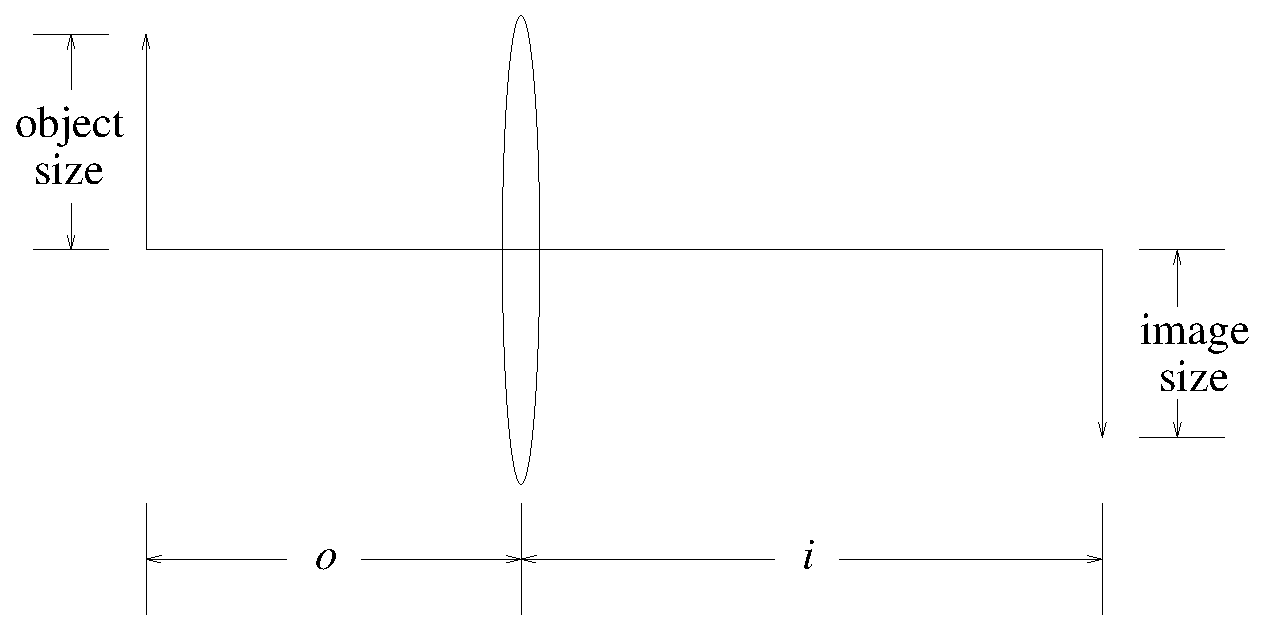
\includegraphics[scale=0.6]{9_imaging/sizes.eps}
\caption{Note the difference between object and image {\it size} and 
{\it distance}.}
\label{fig:opt:sizes}
\end{figure}
The {\it magnification} of a lens is defined as the ratio
\begin{equation}
\fbox{$ \displaystyle m=\frac{\mbox{image size}}{\mbox{object size}}=
\frac{h_{\rm i}}{h_{\rm o}}. $} \label{eq:opt:magdef}
\end{equation}
For thin lenses, we can use the thin lens equation and some geometry to express
the magnification in terms of the object and image {\it distances}
\begin{equation}
\fbox{$ \displaystyle m= -\frac{i}{o}. $} \label{eq:opt:thinlensmag}
\end{equation}
We've introduced a minus sign because of the sign convention for the image 
distance. We leave it up to the student to verify that a {\it positive} 
magnification corresponds to an {\it upright} image, while a {\it negative}
magnification corresponds to an {\it inverted} image.

\section{Apparatus}

For our investigations of imaging optics, we'll use a lamp as a white light 
source which has a crossed arrow slide as an object and two converging lenses 
(one having a focal length of 100~mm and the other of 200~mm).  We'll use
$3''\times 5''$ note cards to find the images produced by our lenses.  All these
will be mounted (using lens holders for the two lenses, and a screen holder for
the note card)  on mobile carriages that will move on an optical bench which
has a scale on one of its sides. 

\vfill
\pagebreak
$$
$$
\vfill
\clearpage
\newpage


%  Label worksheets by \thechapter.W
\renewcommand{\thesection}{\thechapter.W}


\section{Imaging Optics Worksheet}
{\bf \Large Name:}~ \rule{5cm}{.1mm}~~~~~~~
{\bf \Large Day/Time:}~\rule{3cm}{.1mm}\\
{\bf \Large Partner's Name:}~\rule{6cm}{.1mm}\\
\subsection{In-Lab Procedure}
\subsubsection{Focal Length and Magnification of a Lens}

Mount the light source 
at one end of the optical bench followed by
either one 
of the lenses, and the note card.   When you've gotten 
this set-up, it should look like the illustration in 
Figure~\ref{fig:opt:focalsetup}.
\begin{figure}[htb]
\centering 
\epsfxsize=14cm 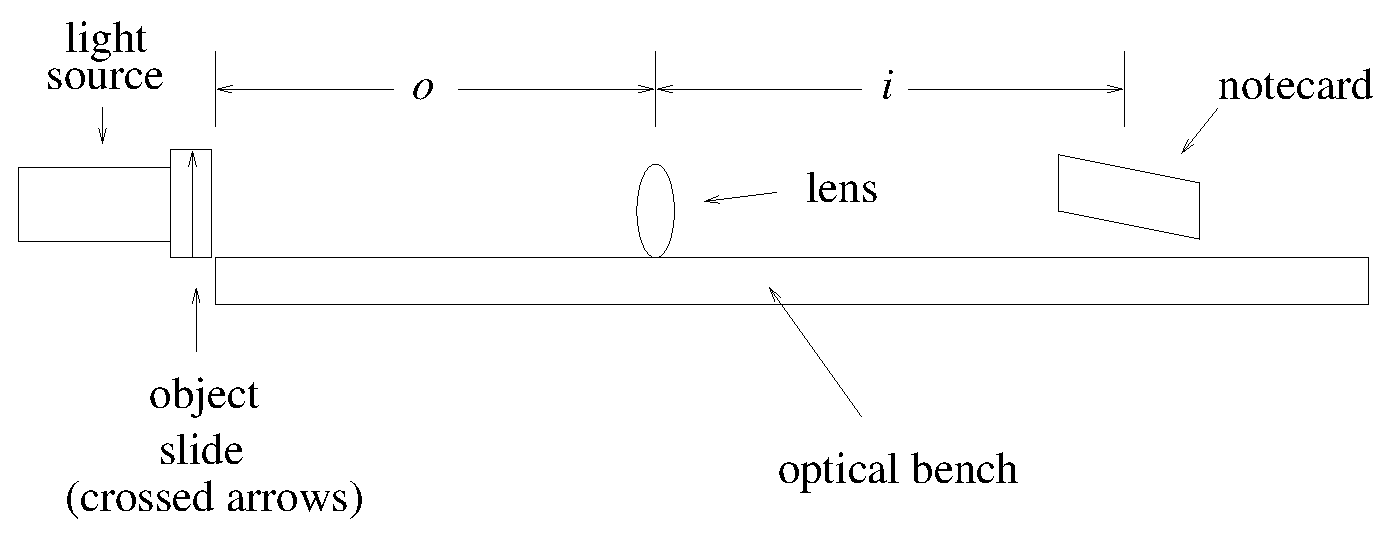
\includegraphics[scale=0.6]{9_imaging/focalsetup.eps}
\caption{The set-up for measurement of focal length.}
\label{fig:opt:focalsetup}
\end{figure}
Refer to the nominal focal length printed on the lens and answer the following questions.  \\
\ \\ 
Place the lens {\bf HALF} its nominal focal length from the object slide. 
Record your answers to the following questions.
\vspace*{.5cm}

\noindent
When you look through the lens, can you see a {\it clear} image of the object?
If you can, is this image upright or inverted?
\vspace*{1.5cm}

\noindent
Are you able to project (through the lens) a {\it clear} image of the object
on the note card? If you are, is this image upright or inverted?
\vspace*{1.5cm}

\noindent
Place the lens {\bf TWICE} its nominal focal length from the object slide. 
Record your answers to the following questions.
\vspace*{.5cm}

\noindent
When you look through the lens, can you see a {\it clear} image of the object?
If you can, is this image upright or inverted?
\vspace*{1.5cm}

\noindent
Are you able to project (through the lens) a {\it clear} image of the object
on the note card? If you are, is this image upright or inverted?

\vspace*{1.5cm}
\noindent
Is all of this consistent with the predictions we made with our ray diagrams? \\
\vspace*{2cm} \\
\newpage
Now make image distance versus object distance measurements for at least five
object-image distance pairs. 
Record your five image distance versus object distance measurements for the
100~mm lens into Table~\ref{tab:OP:136}. For the first pair of measurements,
also measure the image {\it size} and the object {\it size} and record them in
the designated place. Do this by picking two points on one of the arrows;
measure the object size directly from the slide and measure the image size by
marking the note card at the corresponding points on the image and then
measuring the distance with a ruler. Size is positive for a upright image and {\it negative for a inverted image}.
Be sure to include uncertainties. \\
\ \\
\noindent Is the image upright or inverted? \\
\ \\
\begin{table}[t]
\begin{center}
\begin{tabular}{|c|c|c|c|}
\hline
\multicolumn{4}{|c|}{Measurements of $i$ vs. $o$ for ``100 mm'' lens.} \\
\hline
Image Distance ($i$) & Object Distance ($o$) & Image Size & Object Size \\
\hline
\hspace*{3cm} & \hspace*{3cm} & \hspace*{3cm} & \hspace*{3cm} \\
& & &  \\
\hline
& & Leave & Leave  \\
& & Blank& Blank \\
\hline
& & Leave & Leave \\
& & Blank & Blank\\
\hline
& & Leave & Leave \\
& & Blank & Blank \\
\hline
& & Leave & Leave \\
& & Blank & Blank \\
\hline
\end{tabular}
\end{center}
\caption{$i$ vs. $o$ measurements for ``100 mm'' lens.}
\label {tab:OP:136}
\end{table}

% Warning!
%
% If you remove the \newpage command, you may want to fix the instruction to
% use the bottom of the corresponding page for D(1/o) and D(1/i) calculations

\newpage
Repeat the same $i$ versus $o$ measurements with the other lens entering
the data into Table~\ref{tab:OP:238}.  Remember to
make one object and image size measurement as well.
\begin{table}[h]
\begin{center}
\begin{tabular}{|c|c|c|c|}
\hline
\multicolumn{4}{|c|}{Measurements of $i$ vs. $o$ for ``200 mm'' lens.} \\
\hline
Image Distance ($i$) & Object Distance ($o$) & Image Size & Object Size \\
\hline
\hspace*{3cm} & \hspace*{3cm} & \hspace*{3cm} & \hspace*{3cm} \\
& & &  \\
\hline
& & Leave & Leave  \\
& & Blank & Blank \\
\hline
& & Leave & Leave \\
& & Blank & Blank \\
\hline
& & Leave & Leave \\
& & Blank & Blank \\
\hline
& & Leave & Leave \\
& & Blank & Blank \\
\hline
\end{tabular}
\end{center}
\caption{$i$ vs. $o$ measurements for ``200 mm'' lens.}
\label {tab:OP:238}
\end{table}

\subsection{In-Lab Computer Work}
\noindent
Now, plot $1/i$ versus $1/o$ for each lens. You can show your work in
calculating $\Delta(1/o)$ and $\Delta(1/i)$ in the bottom of
page~\pageref{tab:OP:136}. Obtain a weighted least-squares curve fit1 for each
plot. From these fits, determine the focal length of each lens. Record the
slopes and intercepts on the lines below (with uncertainty).

\noindent
{\it ``100~mm'' lens:}
\begin{center}
Slope, $a_1$=~\rule{3cm}{.1mm} ~~~~
Intercept, $b_1$=~\rule{3cm}{.1mm}
\end{center}
\vspace*{.5cm}

\noindent
{\it ``200~mm'' lens:}
\begin{center}
Slope, $a_2$=~\rule{3cm}{.1mm} ~~~~
Intercept, $b_2$=~\rule{3cm}{.1mm}
\end{center}
\vspace*{.5cm}

\subsection{In-Lab Procedure}

\subsubsection{A Compound Lens System} 

\noindent Using both of your lenses, build the configuration shown in 
Figure~\ref{fig:opt:compoundlens}. Place the 100~mm lens at about 50~mm away from the object.\\
%in the step-by-step manner now to be described.\\ 

\begin{figure}[htb]
\centering 
\epsfxsize=9.5cm 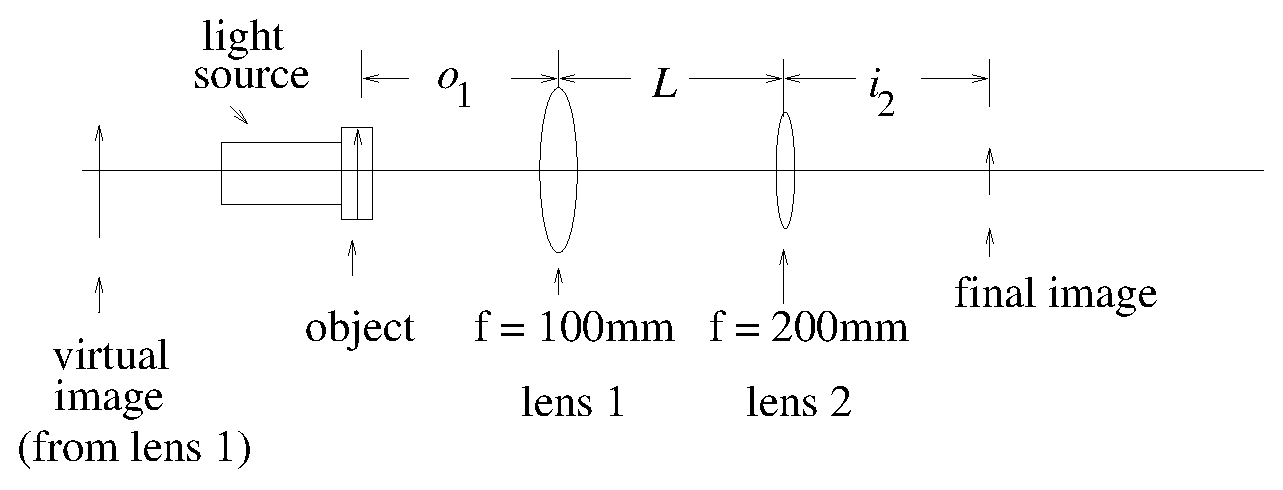
\includegraphics[scale=0.6]{9_imaging/compoundlens.eps}
\caption{A Compound Lens System.}
\label{fig:opt:compoundlens}
\end{figure}

\ \\
%\noindent Is the image real or virtual? \\
%\ \\
%\noindent
%{\it Without uncertainty} for now,  calculate the position of the image of the
%first lens, $i_1$, using the thin lens equation. Do that in two steps. First,
%express the object distance, $o_1$, for that lens in terms of $f_1$ and plug it
%into the thin lens equation to find $i_1$ in terms of $f_1$. Record this
%below. \\
%\vspace*{2cm} \\
%\begin{center}
%$i_1=$~\rule{3cm}{.1mm}
%\end{center}
%\vspace*{.5cm}
%\noindent You can now use the measured focal length, to find a value for $i_1$.

\noindent Measure the object distance $o_1$, distance $L$ and the image distance $i_2$. Record these below
with uncertainties.

\begin{center}
$o_1=$~\rule{3cm}{.1mm}\\
\vspace*{.5cm}
$L=$~\rule{3cm}{.1mm}\\
\vspace*{.5cm}
$i_2=$~\rule{3cm}{.1mm}\\
\end{center}


%\noindent   Place the 200~mm lens at a distance of twice 
%its measured focal length from the {\it calculated position} of the image of 
%the first lens. \\
%\noindent Measure the image distance for the image of the second lens of this
%compound lens system, $i_{comp}.$
%Record this below with uncertainty.

%\begin{center}
%$i_{comp}=$~\rule{3cm}{.1mm}

%\end{center}
\vspace*{.5cm}
\noindent
Measure the original object size $h_o$ and the final image size $h_i$ 
of the compound system.
Record these below with uncertainties.

\begin{center}
$h_o=$~\rule{3cm}{.1mm} ~~~~
$h_i=$~\rule{3cm}{.1mm}
\end{center}


\subsection{Pre-Classroom Checklist}

$\bigcirc$ \hspace*{1cm} Table~\ref{tab:OP:136} with uncertainties and units \\
$\bigcirc$ \hspace*{1cm} Table~\ref{tab:OP:238} with uncertainties and units \\
$\bigcirc$ \hspace*{1cm} Plot of 1/$i$ vs 1/$o$ for 100~mm lens \\
$\bigcirc$ \hspace*{1cm} Plot of 1/$i$ vs 1/$o$ for 200~mm lens \\
$\bigcirc$ \hspace*{1cm} All questions answered 

% \clearpage

\subsection{In-Classroom Calculations \& Analysis}

\subsubsection{Focal Length and Magnification of a Lens}

\noindent What is the slope and the intercept of the $1/i$ versus $1/o$ plot predicted by the thin lens equation?
{\bf SHOW WORK}.
\vspace*{3cm}\\


\noindent From your slope and/or intercept, calculate the measured focal lengths of
each lens, {\it with uncertainties}, and record them below. \\
\vspace*{4cm}\\
\begin{center}
$f_1=$~\rule{3cm}{.1mm} ~~~~
$f_2=$~\rule{3cm}{.1mm}
\end{center}
\clearpage

\noindent
From your image and object sizes, calculate the magnification you measured for
each of the lenses, $m_{100}$ and $m_{200}.$ Record these below with
uncertainties {\bf SHOW WORK}. \\
\vspace*{3cm} 
\begin{center}
$m_{100}=$~\rule{3cm}{.1mm} ~~~~
$m_{200}=$~\rule{3cm}{.1mm}
\end{center}
\vspace*{.5cm}
\noindent 
Now, from the image and object distances in the cases where you measured the
image and object sizes, calculate the {\it predicted} magnification of each lens,
$m'_{100}$ and $m'_{200}.$ Record these below with uncertainties. {\bf SHOW WORK}. \\
\vspace*{3cm} \\
\begin{center}
$m'_{100}=$~\rule{3cm}{.1mm} ~~~~
$m'_{200}=$~\rule{3cm}{.1mm}
\end{center}

\subsubsection{A Compound Lens System}
{\bf Note:} In the procedure of this section, you should use the {\it measured}
focal lengths of the lenses. In other words, {\bf DO NOT} use 100mm and 200mm
as the focal lengths of your lenses. Instead, use the values you have just
determined for $f_{100}$ and $f_{200}.$\\ 

%\vspace*{1cm}
\clearpage
\noindent Calculate the position of the first image; that is, the image distance of the first lens.
The uncertainty is given by
$ \Delta i = \left( \frac{1}{f}-\frac{1}{o} \right)^{-2} \left( \frac{\Delta f}{f^2} + \frac{\Delta o}{o^2} \right)$.\\
\vspace*{3cm} \\

\begin{center}
$i_1=$~\rule{3cm}{.1mm}
\end{center}
\noindent Is the first image real or virtual?\\
\vspace*{.5cm} \\

\noindent Calculate the object distance $o_2$ and the image distance $i_2$ of the second lens.
(Hint: The {\it image} of the first lens act as the {\it object} for the second lens.)
{\bf SHOW WORK}.
\vspace*{1.5cm} \\
\begin{center}
$o_2=$~\rule{3cm}{.1mm}
\vspace*{3cm} \\
$i_2^{(calc)}=$~\rule{3cm}{.1mm}
\end{center}
%\noindent Calculate the magnification of the compound les system.


%Calculate the image distance, $i_2=i'_{comp}$ predicted by the thin lens
%equation for the compound lens system. Follow the same steps that you've taken
%to calculate $i_1$. First express the relevant object distance with respect
%to the corresponding focal length. Plug that expression into the thin lens
%equation to find $i'_{comp}$ in terms of a focal length. Record this result
%below. {\bf SHOW WORK}. \\
%\vspace*{2cm} \\
%\begin{center}
%$i'_{comp}=$~\rule{3cm}{.1mm}
%\end{center}
%\noindent You can now find a value and an uncertainty for $i'_{comp}$, using
%your measured focal length. Show your work and your answer below.
%\vspace*{2cm} \\
%\begin{center}
%$i'_{comp}=$~\rule{3cm}{.1mm}
%\end{center}
\vspace*{.5cm}

\noindent
Calculate the predicted magnification of the compound system, $m'_{comp}$.
Note that $m'_{comp}=m'_{100}\times m'_{200}$, but you
{\bf CANNOT} use the previously determined $m'_{100}$ and $m'_{200}$. You must
calculate the new individual magnifications from the given and derived
$o_1, i_1, o_2$, and $i_2$ of each lens in the compound system. \\
\vspace*{2cm} \\
\begin{center}
$m'_{comp}=$~\rule{3cm}{.1mm} \\
\end{center}
\noindent 
Using the final image and original object sizes you measured, 
calculate the magnification 
of the final image, $m_{comp}.$ 
Show work. \\
\vspace*{3cm} 
\begin{center}
$m_{comp}=$~\rule{3cm}{.1mm} ~~~~
\end{center}


\subsection{In-Classroom Discussion}
\subsubsection{Focal Length and Magnification of a Lens}
Consider the image(s) you were able to observe when the lens was half its
nominal focal length from the object slide. Were they real or virtual?
\vspace*{.3cm}

\noindent
Consider the image(s) you were able to observe when the lens was twice its
nominal focal length from the object slide. Were they real or virtual?
\vspace*{.3cm}


\noindent
Compare the slopes of each of your plots to the slope predicted by the thin lens
equation.
\vspace*{2.4cm}

\noindent 
Compare the nominal focal lengths of each of your lenses to the measured
values.
\vspace*{2.4cm}

\noindent
Compare the measured magnifications of each of your lenses to the predicted
values.
\vspace*{2.4cm}

\noindent
Is the sign convention for magnification consistent with your observations?
\vspace*{2.3cm}



\subsubsection{A Compound Lens System}  

%Is the image of the first lens alone real or virtual? \\
%\vspace*{.3cm} 

\noindent
Compare the image distance you measured for the compound lens system,
$i_2,$ to the predicted image distance $i_2^{(calc)}.$ \\
\vspace*{4cm} 

\noindent
Compare the magnification you predicted  for the compound lens system,
$m'_{comp}$, with the measured magnification, $m_{comp}$. \\
%\vspace*{3cm} 

\newpage
\subsection{In-Classroom Conclusion}

Write a {\it brief} (that is, a one or two paragraph) conclusion for
this lab. In it, you should summarize the physical
principles which were meant to be illustrated in this experiment. You
should also describe the degree to which your data supported these
principles.



\vfill
{\Large End Worksheet} 
% Go back to ordinary section numbering
\renewcommand{\thesection}{\thechapter.\arabic{section}}


















